% Figure 2, traced from the original printed diagram on page 14.
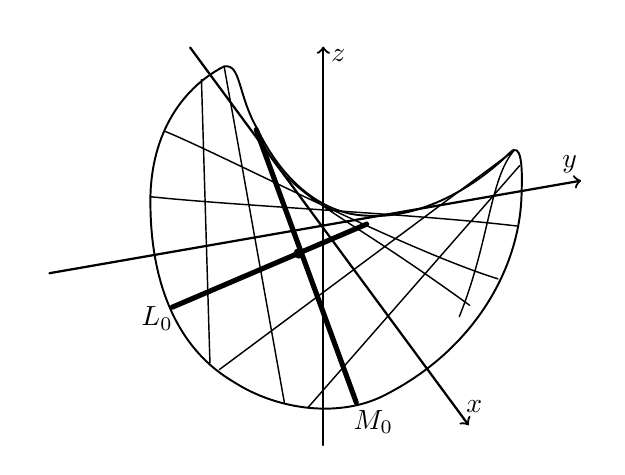
\begin{tikzpicture}[x=.34bp,y=-.34bp,line width=.52bp,line cap=round,line join=round]
  \path[use as bounding box] (0,0) rectangle (603,444);
  % The outline and characteristic rulings of the surface.
  \draw[line width=.7bp] (208,41) .. controls (226,38) and (222,70) .. (243,107)
    .. controls (269,161) and (310,197) .. (358,199)
    .. controls (411,203) and (468,174) .. (510,133)
    .. controls (523,119) and (524,148) .. (523,174)
    .. controls (522,255) and (472,340) .. (382,387)
    .. controls (334,414) and (266,406) .. (218,375)
    .. controls (155,338) and (131,266) .. (130,190)
    .. controls (128,117) and (161,65) .. (208,41) -- cycle;
  \draw (184,55)--(193,355)
        (208,41)--(272,398)
        (146,110).. controls (207,135) and (396,234) .. (498,266)
        (130,179).. controls (225,189) and (409,197) .. (518,210)
        (203,362)--(511,133)
        (297,402)--(521,146)
        (244,112).. controls (275,181) and (314,182) .. (468,294)
        (457,306).. controls (489,227) and (489,160) .. (515,130);
  \draw[line width=1.85bp] (153,296)--(359,208);
  \draw[line width=1.85bp] (242,108)--(348,397);
  % Coordinate axes and their labels.
  \draw[line width=.81bp,->] (23,260)--(586,162);
  \draw[line width=.81bp,->] (313,442)--(313,20);
  \draw[line width=.81bp,->] (172,21)--(467,421);
  \fill (287,239) circle[radius=1.9bp];
  \node[inner sep=0pt] at (473,401) {$x$};
  \node[inner sep=0pt] at (574,145) {$y$};
  \node[inner sep=0pt] at (329,29) {$z$};
  \node[inner sep=0pt] at (137,308) {$L_0$};
  \node[inner sep=0pt] at (366,418) {$M_0$};
\end{tikzpicture}
